% Created 2024-04-20 Σαβ 19:23
% Intended LaTeX compiler: pdflatex
\documentclass[11pt]{article}
\usepackage[utf8]{inputenc}
\usepackage[T1]{fontenc}
\usepackage{graphicx}
\usepackage{longtable}
\usepackage{wrapfig}
\usepackage{rotating}
\usepackage[normalem]{ulem}
\usepackage{amsmath}
\usepackage{amssymb}
\usepackage{capt-of}
\usepackage{hyperref}
\usepackage{booktabs}
\usepackage{import}
\usepackage[LGR, T1]{fontenc}
\usepackage[greek, english, american]{babel}
\usepackage{alphabeta}
\usepackage{esint}
\usepackage{mathtools}
\usepackage{esdiff}
\usepackage{makeidx}
\usepackage{glossaries}
\usepackage{newfloat}
\usepackage{minted}
\usepackage[a4paper, margin=3cm]{geometry}
\usepackage{chemfig}
\usepackage{svg}
\author{Vidianos Giannitsis}
\date{\today}
\title{ΒΙΟΑΠΟΔΟΜΗΣΗ ΥΠΟΛΕΙΜΜΑΤΩΝ ΤΡΟΦΙΜΩΝ ΚΑΙ ΠΑΡΑΓΩΓΗ ΒΙΟΑΕΡΙΟΥ ΜΕΣΩ ΑΝΑΕΡΟΒΙΑΣ ΧΩΝΕΥΣΗΣ ΣΕ ΕΡΓΑΣΤΗΡΙΑΚΗ ΚΑΙ ΠΙΛΟΤΙΚΗ ΚΛΙΜΑΚΑ}
\hypersetup{
 pdfauthor={Vidianos Giannitsis},
 pdftitle={ΒΙΟΑΠΟΔΟΜΗΣΗ ΥΠΟΛΕΙΜΜΑΤΩΝ ΤΡΟΦΙΜΩΝ ΚΑΙ ΠΑΡΑΓΩΓΗ ΒΙΟΑΕΡΙΟΥ ΜΕΣΩ ΑΝΑΕΡΟΒΙΑΣ ΧΩΝΕΥΣΗΣ ΣΕ ΕΡΓΑΣΤΗΡΙΑΚΗ ΚΑΙ ΠΙΛΟΤΙΚΗ ΚΛΙΜΑΚΑ},
 pdfkeywords={},
 pdfsubject={},
 pdfcreator={Emacs 29.3 (Org mode 9.6.15)}, 
 pdflang={English}}
\makeatletter
\newcommand{\citeprocitem}[2]{\hyper@linkstart{cite}{citeproc_bib_item_#1}#2\hyper@linkend}
\makeatother

\usepackage[notquote]{hanging}
\begin{document}

\maketitle
\tableofcontents


\section{Μεθοδολογία}
\label{sec:org01c1556}
\subsection{Συλλογή και προεπεξεργασία υποστρώματος}
\label{sec:org108372b}
Τα υπολείμματα τροφών (FW) που χρησιμοποιήθηκαν για τα πειράματα εργαστηριακής κλίμακας συλλέχθηκαν από το εστιατόριο του Εθνικού Μετσόβιου Πολυτεχνείου. Αρχικά, αντικείμενα όπως κόκκαλα, χαρτί και άλλα αφαιρέθηκαν από τα υπολείμματα. Έπειτα, τα τρόφιμα τεμαχίστηκαν σε μπλέντερ (Cecotec Powder Black Titanium 2000) για να δημιουργηθεί μία ομοιόμορφη ημιστερεή φάση η οποία μπορεί να χρησιμοποιηθεί ως υπόστρωμα για την υδρόλυση. Το υλικό αυτό αποθηκεύτηκε σε κατάψυξη στους - 20 \(^oC\) για περαίτερω χρήση.

Για τα πειράματα πιλοτικής κλίμακας, ακολουθήθηκε μία παρόμοια διαδικασία, με βασική διαφορά ότι δεν υπήρχε απαίτηση σε τεμαχισμό καθώς ο ίδιος ο αντιδραστήρας είχε την δυνατότητα αυτή.

\subsection{Εμβόλιο}
\label{sec:orgfbf78e3}
Για την βιοαποδόμηση της οργανικής ύλης χρησιμοποιήθηκε εμπορικό σκεύασμα ενζύμων και μικροοργανισμών (Ένζυμα PROGEN \url{https://www.progen-enzymes.com/}) το οποίο έχει ως σκοπό την αποτελεσματική υδρόλυση του υποστρώματος αλλά και την ζύμωση της οργανικής ύλης που περιέχει σε πτητικά λιπαρά οξέα (VFAs).

Για την αναερόβια χώνευση χρησιμοποιήθηκε λάσπη από 2 διαφορετικές πηγές (++ αλλά εγώ δεν ξέρω άλλες πληροφορίες).

\subsection{Βιοαποδόμηση υπολειμμάτων τροφών - Εργαστηριακή Κλίμακα}
\label{sec:orga1131ed}
Τα πειράματα βιοαποδόμησης σε εργαστηριακή κλίμακα ήταν διαλείποντος έργου και έγιναν σε όργανο το οποίο έχει 7 διαθέσιμα δοχεία συνολικού όγκου 1000 ml εξοπλισμένα με αναδευτήρες και με δυνατότητα ρύθμισης της θερμοκρασίας. Το σύστημα αυτό προσφέρει την δυνατότητα να δοκιμαστούν αρκετές συνθήκες σε κάθε πείραμα, με βασικό περιορισμό ότι η ρύθμιση της θερμοκρασίας είναι κεντρική και όλα τα δοχεία λειτουργούν στην ίδια θερμοκρασία.

(λογικά μία φωτογραφία)

Ο βασικός πειραματικός σχεδιασμός που έγινε για την βελτιστοποίηση της διεργασίας χρησιμοποιήσε 2 θερμοκρασίες της μεσόφιλης περιοχής, τους 35 \(^oC\) και τους 40 \(^oC\). Σε κάθε δοχείο τροφοδοτήθηκαν 200 g τεμαχισμένων υπολειμμάτων τροφών και αυτά αραιώθηκαν με 600 ml νερό. Η αραίωση αυτή επιλέχθηκε μετά από κάποια προπαρασκευαστικά πειράματα ως μία τιμή στην οποία πετυχαίνεται καλή ομοιογένια του υποστρώματος και τα στερεά δεν δημιουργούν κάποιο πρόβλημα. Κάθε δοχείο είχε προσθήκη διαφορετικής ποσότητας του σκευάσματος ενζύμων και μικροοργανισμών (μιξ) με τις τιμές που εξετάστηκαν να είναι 0 ml (επίδραση μόνο της θερμοκρασίας), 1 ml, 2 ml, 4 ml και 8 ml. Οπότε δημιουργήθηκαν αναλογίες υποστρώματος:εμβολίου 200, 100, 50 και 25 g υγρού FW ανά ml μιξ. Η ανάδευση ρυθμίστηκε στα 120 rpm για κάθε πείραμα.

\subsection{Βιοαποδόμηση υπολειμμάτων τροφών - Πιλοτική Κλιμάκα}
\label{sec:org55f640a}
Για τα πειράματα σε πιλοτική κλίμακα χρησιμοποιήθηκε ο αερόβιος χωνευτήρας ORCA (\url{https://www.feedtheorca.com/}). Η λειτουργία του αντιδραστήρα ήταν ημι-συνεχής καθώς η τροφοδοσία γινόταν 2 φορές την ημέρα (μία το πρωί και μία το απόγευμα) με ποσότητα περίπου στα 30-40 kg υγρού FW/ημέρα. Η εκροή του αντιδραστήρα συλλεγόταν σε δεξαμενή συνολικής χωρητικότητας 250 L μετά από λιποσυλλογή.

Ο αντιδραστήρας έχει πληρωτικό υλικό, το οποίο επιτρέπει την πιο αποτελεσματική διεξαγωγή της αντίδρασης. Επίσης, έχει εσωτερική ζυγαριά για την μέτρηση της μάζας της τροφοδοσίας του και ροόμετρο για την μέτρηση της παροχής στην εκροή. Τέλος, έχει ένα PLC το οποίο επιτρέπει την ρύθμιση του ρυθμού τροφοδοσίας του ενζυμικού σκευάσματος καθώς και τη ρύθμιση του νερού που προστίθεται είτε στο εσωτερικό του αντιδραστήρα ή στην εκροή (για να γίνει καλύτερη αραίωση του συστήματος).

Στα πειράματα που έγιναν εξετάστηκε η επίδραση όλων αυτών των παραμέτρων.

\subsection{Αναερόβια Χώνευση}
\label{sec:orgb9e7f92}
Η αναερόβια χώνευση έγινε σε εργαστηριακή κλίμακα χρησιμοποιώντας μία batch διάταξη μέτρησης του μεθανίου που μπορεί να παράξει το υδρόλυμα. Χρησιμοποιήθηκαν δοχεία συνολικού όγκου 500 ml τα οποία τοποθετήθηκαν σε θερμόλουτρο ρυθμισμένο στους 37 \(^oC\) με ανάδευση 170 rpm. Τα δοχεία σφραγίστηκαν με σιλικόνη για να μην υπάρξουν διαρροές. Το παραγώμενο αέριο αρχικά διοχετεύεται σε διάλυμα καυστικού νατρίου για δέσμευση του διοξειδίου του άνθρακα ενώ το μεθάνιο περνάει σε μία προχοίδα όπου με μέτρηση της μετατόπισης του υγρού υπολογίζεται η παραγωγή αερίου. Η μετατόπιση αυτή καταγράφεται με χρήση κάμερας που υπάρχει στην διάταξη.

Αρχικά, η αναερόβια λάσπη ενεργοποιήθηκε με τροφοδοσία με οξικό οξύ και έπειτα έγινε τροφοδοσία με τα παραγώμενα υδρολύματα. Εκτός από τα υδρολύματα, έγινε και μία τροφοδοσία με ανεπεξέργαστο FW για να παρατηρηθεί αν η διεργασία βιοαποδόμησης βοήθησε στην πιο αποτελεσματική χώνευση. Σε όλα τα πειράματα που έγιναν, η τροφοδοσία υποστρώματος ήταν 100 mg COD. Στον κύκλο με την πρώτη λάσπη, τροφοδοτήθηκαν 1.55 g VS λάσπης, οδηγώντας σε μία αναλογία υποστρώματος:εμβολίου 0.06 ενώ στον δεύτερο τροφοδοτήθηκαν 4.2 g VS λάσπης και άρα μία αναλογία 0.02. Η αναλογίες αυτές είναι γενικά χαμηλές, με σκοπό να υπάρχει μία γρήγορη απόκριση στην τροφοδοσία και να μην παραχθεί πολύ μεγάλη ποσότητα αερίου, καθώς οι προχοίδες που χρησιμοποιούνται έχουν χωρητικότητα 50 ml.

Καθώς η καταγραφή του όγκου ήταν 24ωρη, έγινε και κινητική ανάλυση της παραγωγής μεθανίου, με χρήση του τροποποιημένου μοντέλου Gompertz (\citeprocitem{4}{Zwietering et al. 1990}) το οποίο έχει χρησιμοποιηθεί εκτενώς στη βιβλιογραφία για την ανάλυση αυτή (\citeprocitem{3}{Uçkun Kiran, Trzcinski, and Liu 2015}; \citeprocitem{1}{Feng et al. 2020}; \citeprocitem{2}{Hobbs et al. 2018}).

\begin{equation}
\tag{1}
P(t) = P_{\max } \exp \left( - \exp \left[ \frac{R_{\max }e (λ-t)}{P_{\max }} + 1 \right] \right)
\label{eqn:1}
\end{equation}

Το μοντέλο αυτό έχει τρείς παραμέτρους. Τη μέγιστη δυνατή παραγωγή μεθανίου \(P_{\max }\), τον μέγιστο ειδικό ρυθμό παραγωγής μεθανίου \(R_{\max }\) και τον χρόνο καθυστέρησης \(λ\). 

\section{Αποτελέσματα/Συμπεράσματα}
\label{sec:org39a13e2}
\subsection{Βιοαποδόμηση υπολειμμάτων τροφών}
\label{sec:org9584260}
Η διαδικασία της βιοαποδόμησης, η οποία είναι στην ουσία συνδυασμός δύο διεργασιών, μίας υδρόλυσης και μίας ζύμωσης είναι μία περίπλοκη διεργασία στην ανάλυση. Αρχικά αυξάνεται το COD καθώς διαλυτοποιείται η οργανική ύλη, αλλά ταυτόχρονα, αυτή καταναλώνεται από τους μικροοργανισμούς, είτε για την ανάπτυξη τους ή για την παραγωγή κάποιου μεταβολικού προιόντος. Όσο περισσότερο μιξ προστίθεται, τόσο πιο αποτελεσματικά γίνεται η ζύμωση, με αποτέλεσμα μεγαλύτερη μείωση του COD, αλλά παραγωγή περισσότερων μεταβολικών προιόντων. Βέβαια, παρατηρήθηκε πως μετά από μία ποσότητα, η διεργασία της ζύμωσης φτάνει σε κορεσμό και δεν μπορεί να βελτιωθεί περαιτέρω, οπότε, οι μεγάλες ποσότητες μιξ (4 και 8 ml) είχαν αμελητέο ή αρνητικό αποτέλεσμα στην συνολική διεργασία.

Παρακάτω παρουσιάζονται τα βασικά αποτελέσματα του πειραματικού κύκλου αυτού. Αυτά είναι η ποσότητα και η αναλογία των προιόντων σε κάθε εκροή, ο βαθμός οξίνισης κάθε συστήματος (ο οποίος ορίζεται ως το ποσοστό του διαλυτού COD που οφείλεται σε προιόντα οξεογένεσης), το ποσοστό των αρχικών σακχάρων που μετατράπηκαν σε προιόντα οξεογένεσης και τέλος τα αποτελέσματα μίας ανάλυσης ευαισθησίας.

\begin{figure}[htbp]
\centering
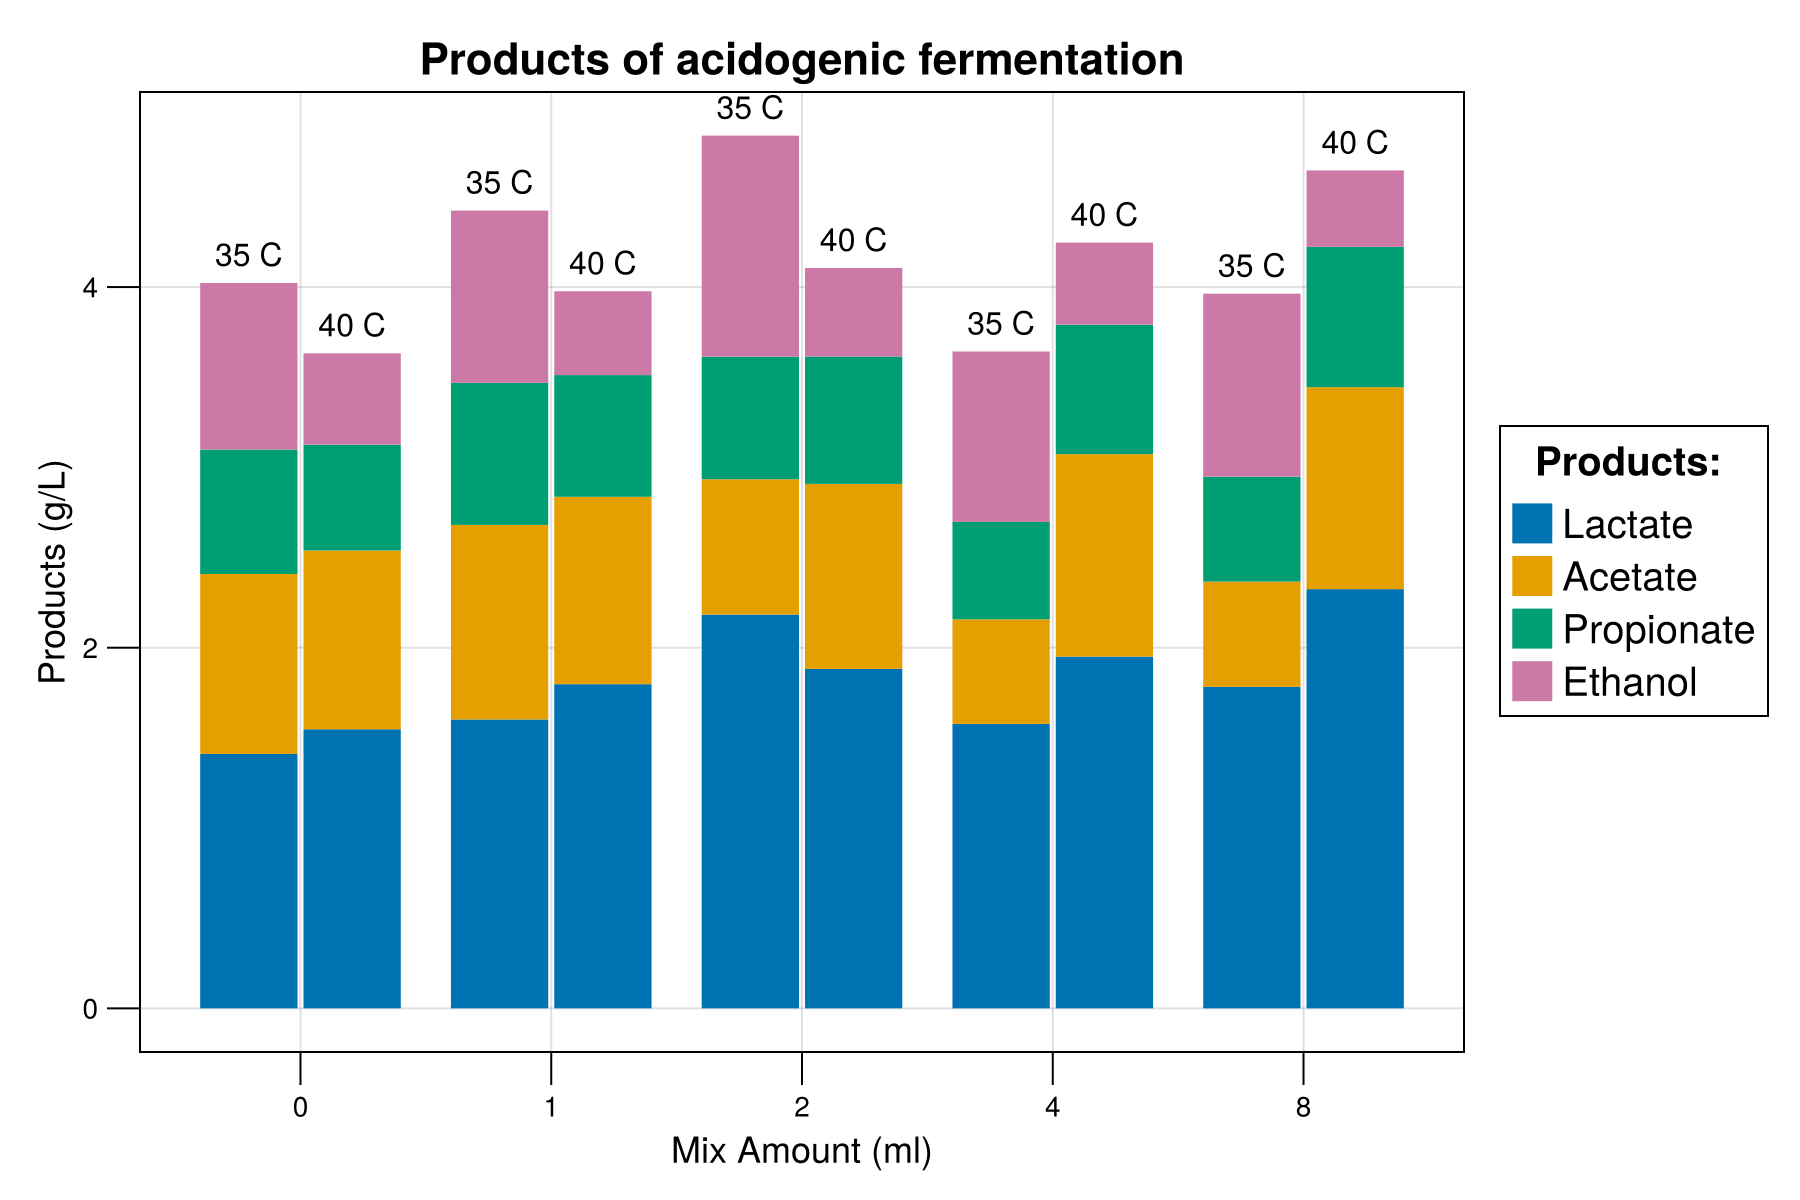
\includegraphics[width=.9\linewidth]{../plots/35_40_comp/final_products.png}
\caption{Κατανομή προιόντων Οξεογένεσης}
\end{figure}

\begin{figure}[htbp]
\centering
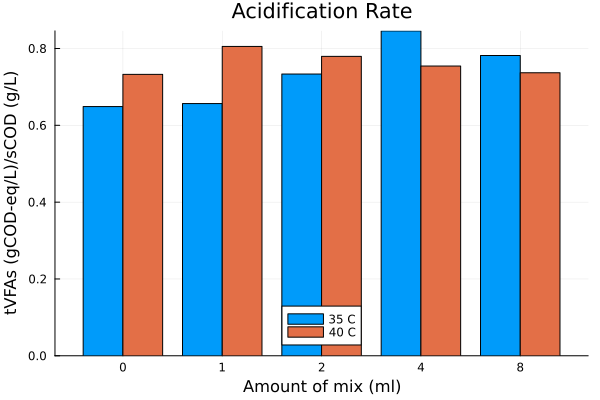
\includegraphics[width=.9\linewidth]{../plots/35_40_comp/acidification_comp.png}
\caption{Βαθμός Οξίνισης}
\end{figure}

\begin{equation}
\tag{2}
Yield = \frac{Prod_{\text{final}} - Prod_{\text{init}}}{Sugars_{init}}
\label{eqn:2}
\end{equation}

\begin{figure}[htbp]
\centering
\includegraphics[width=.9\linewidth]{../plots/35_40_comp/Δprod.png}
\caption{Ποσοστό σακχάρων που μετατράπηκαν σε προιόντα}
\end{figure}

\begin{figure}[htbp]
\centering
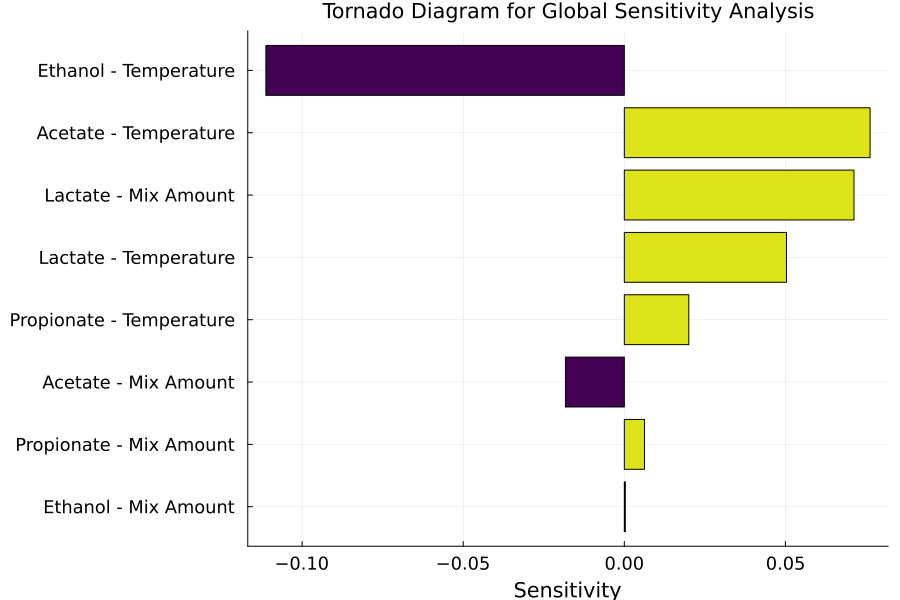
\includegraphics[width=.9\linewidth]{../plots/sensitivity/global_tornado.png}
\caption{Ανάλυση Ευαισθησίας}
\end{figure}

Εκτός από αυτό το διάγραμμα, έχει ιδιαίτερο ενδιαφέρον να περιορίσουμε την ανάλυση ευαισθησίας στην περιοχή 2-8 ml του μιξ, όπου θα δούμε πως το σύστημα πιάνει ένα "πλατό" και δεν συνεισφέρει ιδιαίτερα η περαιτέρω προσθήκη.

\begin{center}
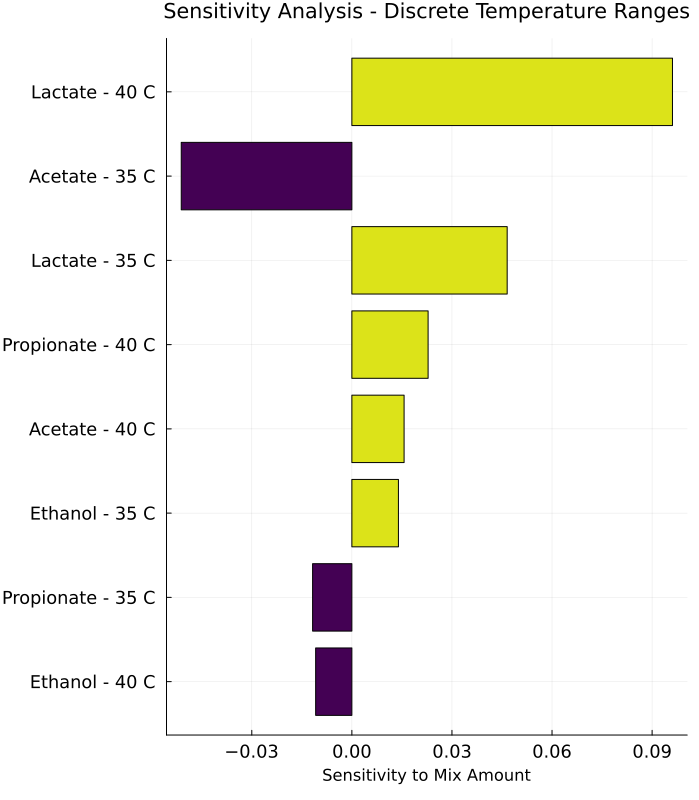
\includegraphics[width=.9\linewidth]{../plots/sensitivity/temperature_tornado.png}
\end{center}

Από άποψη θερμοκρασίας, αποφασίστηκε πως οι 40 \(^oC\) είναι πιο αποτελεσματικοί, με κύρια κριτήρια ότι η μετατροπή των σακχάρων σε προιόντα είναι πιο αποτελεσματική και ότι το οξικό οξύ, το οποίο είναι το ιδανικό υπόστρωμα για την αναερόβια χώνευση έχει ισχυρή θετική επίδραση στην αύξηση της θερμοκρασίας από 35 σε 40 \(^oC\).

Από την άποψη της ποσότητας του μιξ που θα προσθέσουμε, φαίνεται πως γίνεται καλύτερη ζύμωση με την προσθήκη του (το οποίο φαίνεται ειδικά από τον βαθμό οξίνισης) αλλά πως οι μεγάλες ποσότητες (πάνω από 2 ml) δεν προσέφεραν κάτι στην ζύμωση.

Το υπόστρωμα που χρησιμοποιήθηκε για τα πειράματα αυτά είχε σχετικά χαμηλό COD πολλών υδρολυμάτων στην διάταξη της αναερόβιας χώνευσης, αποφασίστηκε να δοκιμαστούν οι ποσότητες 0, 1, 2 και 4 ml για την απόδοση τους στην αναερόβια χώνευση.

Ένα πρόβλημα είναι πω το υπόστρωμα που χρησιμοποιήθηκε για τα πειράματα αυτά είχε σχετικά χαμηλό COD και λίγα στερεά καθώς ήταν κυρίως λαχανικά. Για την αναερόβια χώνευση έγινε ένα καινούργιο πείραμα βιοαποδόμησης, στο οποίο χρησιμοποιήθηκε υπόστρωμα με μεγαλύτερο COD. Σε αυτό, παρατηρήθηκε μία τάση στα COD η οποία δεν είχε παρατηρηθεί στα προηγούμενα πειράματα και είναι ενδεικτική της υδρόλυσης.

\begin{center}
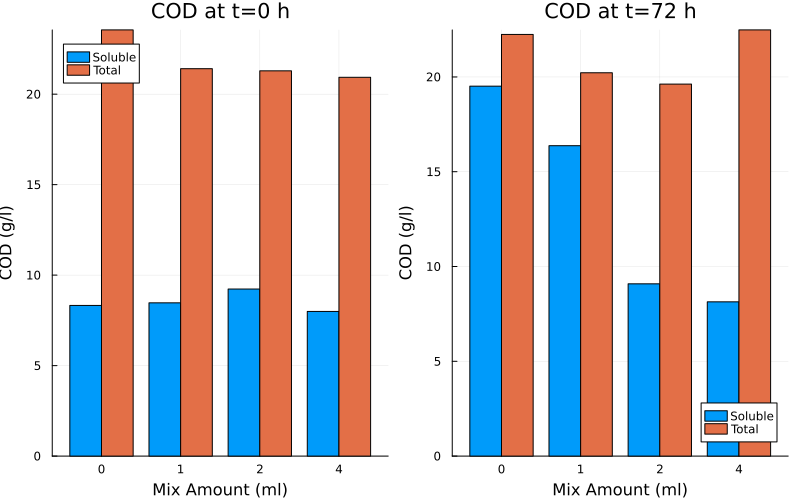
\includegraphics[width=.9\linewidth]{../plots/26_03/complete_cod_bar_26_03.png}
\end{center}

Φαίνεται πως όσο περισσότερο μιξ προστίθεται, τόσο μειώνεται το COD, το οποίο είναι λογικό καθώς γίνεται υδρόλυση, αλλά επίσης καλύτερη ζύμωση. 

Οπότε, έγιναν πειράματα αναερόβιας χώνευσης και με τα 4 αυτά υδρολύματα για να διαπιστωθεί τι επιδρά περισσότερο στην χώνευση. Η πιο αποτελεσματική ζύμωση που πετυχαίνει η προσθήκη του μιξ αυτού ή μία βιοαποδόμηση ρυθμίζοντας μόνο την θερμοκρασία, στην οποία γίνεται καλή υδρόλυση και αύξηση του COD αλλά με λιγότερο ποιοτική ζύμωση.

\subsection{Αναερόβια Χώνευση}
\label{sec:org23c2e1f}
Η αναερόβια χώνευση με τα υδρολύματα ήταν αποτελεσματική καθώς όλα τα δείγματα παρήγαγαν μεθάνιο. Όμως, υπήρχε ξεκάθαρη διαφορά μεταξύ τους, το οποίο δείχνει πως η βιοαποδόμηση που έγινε έπαιξε ρόλο για την αναερόβια χώνευση.

\begin{figure}[htbp]
\centering
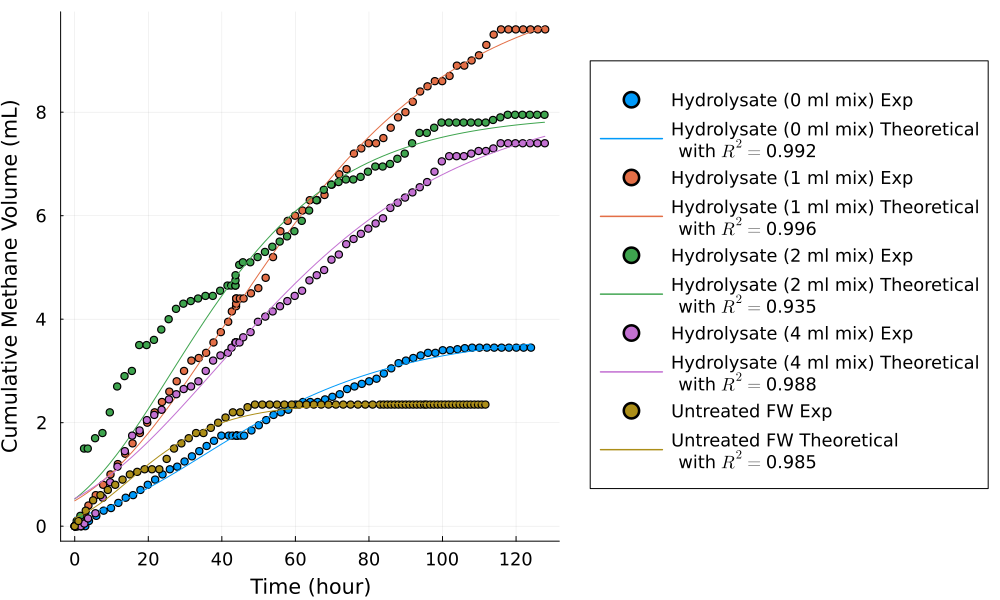
\includegraphics[width=.9\linewidth]{../plots/BMPs/methane_s1_r2_comp.png}
\caption{Αποτελέσματα πρώτου κύκλου αναερόβιας χώνευσης}
\end{figure}

Από το παραπάνω διάγραμμα φαίνεται πως η προσαρμογή του μοντέλου Gompertz ήταν καλή σε όλα τα πειράματα, ενώ μπορούν να βγούν κάποια συμπεράσματα για την επίδραση της προεπεξεργασίας στην χώνευση.

\begin{itemize}
\item Τα υπολείμματα τροφών δεν μπορούν να παράξουν μεγάλη ποσότητα μεθανίου χωρίς προεπεξεργασία. Μετά από μέτρηση του τελικού pH στον αντιδραστήρα αυτόν, βρέθηκε πως το πρόβλημα ήταν η υπερβολική οξίνιση του αντιδραστήρα καθώς είχε φτάσει pH 4.22 όπου δεν μπορεί πλέον να συνεχίσει η χώνευση. Αυτό είναι ένα συχνό πρόβλημα στην αναερόβια χώνευση, ειδικά για όξινα απόβλητα όπως τα υπολείμματα τροφών. Ο διαχωρισμός των σταδίων της υδρόλυσης και οξεογένεσης, όπως προτείνεται στην μελέτη αυτή συνεισφέρει σημαντικά στην επίλυση του.
\item Το πείραμα χωρίς την προσθήκη του ενζυμικού σκευάσματος είχε και αυτό κακή απόδοση, το οποίο δείχνει πως δεν μπορεί να γίνει καλή βιοαποδόμηση ρυθμίζοντας μόνο την θερμοκρασία.
\item Τα 2 καλύτερα πειράματα είναι αυτό με 1 ml μιξ και αυτό 2 ml. Η βασική διαφορά, όπως φάνηκε και από τις παραμέτρους των μοντέλων είναι πως το υδρόλυμα με 1 ml μιξ είχε μεγαλύτερο χρόνο καθυστέρησης. Αυτό δείχνει πως το 2 είχε καλύτερη οξεογένεση κατά την διεργασία βιοαποδόμησης, το οποίο συνάδει με τα παραπάνω συμπεράσματα. Όμως, το υδρόλυμα με 1 ml μιξ είχε υψηλότερο COD επειδή η μικρότερη ποσότητα μιξ συντέλεσε στην διεργασία να είναι περισσότερο υδρόλυση παρά ζύμωση. Έτσι, μόλις ολοκληρωθεί η οξεογένεση στο δείγμα αυτό και φτάσει στον μέγιστο ρυθμό παραγωγής μεθανίου του, ξεπερνάει την απόδοση του υδρολύματος με 2 ml μιξ. Οπότε θεωρείται και το καλύτερο πείραμα.
\end{itemize}

Όμως, σε όλους τους αντιδραστήρες στο πείραμα αυτό υπήρχε μία σχετικά χαμηλή παραγωγικότητα μεθανίου, το οποίο οδήγησε στην υπόθεση πως η λάσπη που χρησιμοποιήθηκε δεν είναι ιδιαίτερα ενεργή. Οπότε, έγινε ένας δεύτερος κύκλος πειραμάτων με μία πιο ενεργή λάσπη για να εξεταστεί αν μπορούν να επαναληφθούν τα αποτελέσματα αυτά.
\section{Βιβλιογραφία}
\label{sec:org511b220}
\begin{hangparas}{1.5em}{1}
\hypertarget{citeproc_bib_item_1}{Feng, Kai, Huan Li, Zhou Deng, Qiao Wang, Yangyang Zhang, and Chengzhi Zheng. 2020. “Effect of Pre-Fermentation Types on the Potential of Methane Production and Energy Recovery from Food Waste.” \textit{Renewable Energy} 146 (February): 1588–95. \url{https://doi.org/10.1016/j.renene.2019.07.127}.}

\hypertarget{citeproc_bib_item_2}{Hobbs, S.R., A.E. Landis, B.E. Rittmann, M.N. Young, and P. Parameswaran. 2018. “Enhancing Anaerobic Digestion of Food Waste through Biochemical Methane Potential Assays at Different Substrate: Inoculum Ratios.” \textit{Waste Management} 71: 612–17. \url{https://doi.org/10.1016/j.wasman.2017.06.029}.}

\hypertarget{citeproc_bib_item_3}{Uçkun Kiran, Esra, Antoine P. Trzcinski, and Yu Liu. 2015. “Enhancing the Hydrolysis and Methane Production Potential of Mixed Food Waste by an Effective Enzymatic Pretreatment.” \textit{Bioresource Technology} 183 (May): 47–52. \url{https://doi.org/10.1016/j.biortech.2015.02.033}.}

\hypertarget{citeproc_bib_item_4}{Zwietering, M. H., I. Jongenburger, F. M. Rombouts, and K. van ’t Riet. 1990. “Modeling of the Bacterial Growth Curve.” \textit{Applied and Environmental Microbiology} 56 (6): 1875–81. \url{https://doi.org/10.1128/aem.56.6.1875-1881.1990}.}\bigskip
\end{hangparas}
\end{document}
